\section{Εφαρμογή με 2 σένσορες και έναν ενεργοποιητή}
\label{sec:example1}

Σε αυτό το παράδειγμα αναλύεται η χρήση των παραπάνω εργαλείων για την ανάπτυξη μιας εφαρμογής για τη λήψη διαφόρων μετρήσεων από περιφερειακά. Το σύστημα αποτελείται από έναν μικροελεγκτή NodeMCU ESP32 που αποτελεί την κύρια υπολογιστική μονάδα, ένα σόναρ, έναν αισθητήρα περιβάλλοντος και έναν ενεργοποιητή με LED. Επίσης, χρησιμοποιείται και ένα raspberry pi στο οποίο τρέχει ένας broker. Οι συνδέσεις μεταξύ των συσκευών ορίστηκαν σε ένα αρχείο\footnote{\url{https://github.com/robotics-4-all/2020_riot_mde_thanos_manolis/blob/master/test_connections/example1.con}}, χρησιμοποιώντας τη γλώσσα που αναλύεται στην \autoref{subsec:syntax_connections}.

Για την παραγωγή του κώδικα εκτελέστηκε η παρακάτω εντολή.

\begin{lstlisting}
$ riot_mde --connections example1.con
\end{lstlisting}

Όπου example1.con είναι το όνομα του αρχείου περιγραφής συνδέσεων μεταξύ των συσκευών. Με την εκτέλεση της εντολής αυτής, παράγεται ένα αρχείο κώδικα C, ένα Makefile, μία εικόνα όπου φαίνεται η συνδεσμολογία των συσκευών και μια εικόνα όπου φαίνονται όλα τα χαρακτηριστικά του μοντέλου των συνδέσεων. Τα αρχεία δημιουργήθηκαν σύμφωνα με τα πρότυπα αρχεία που αναλύθηκαν στην \autoref{subsec:c_code}.

Στο \autoref{fig:example_connections} απεικονίζεται η συνδεσμολογία. Το δεύτερο διάγραμμα που παράχθηκε παρουσιάζεται στο \autoref{fig:connections_model}.

\begin{figure}[!ht]
	\centering
	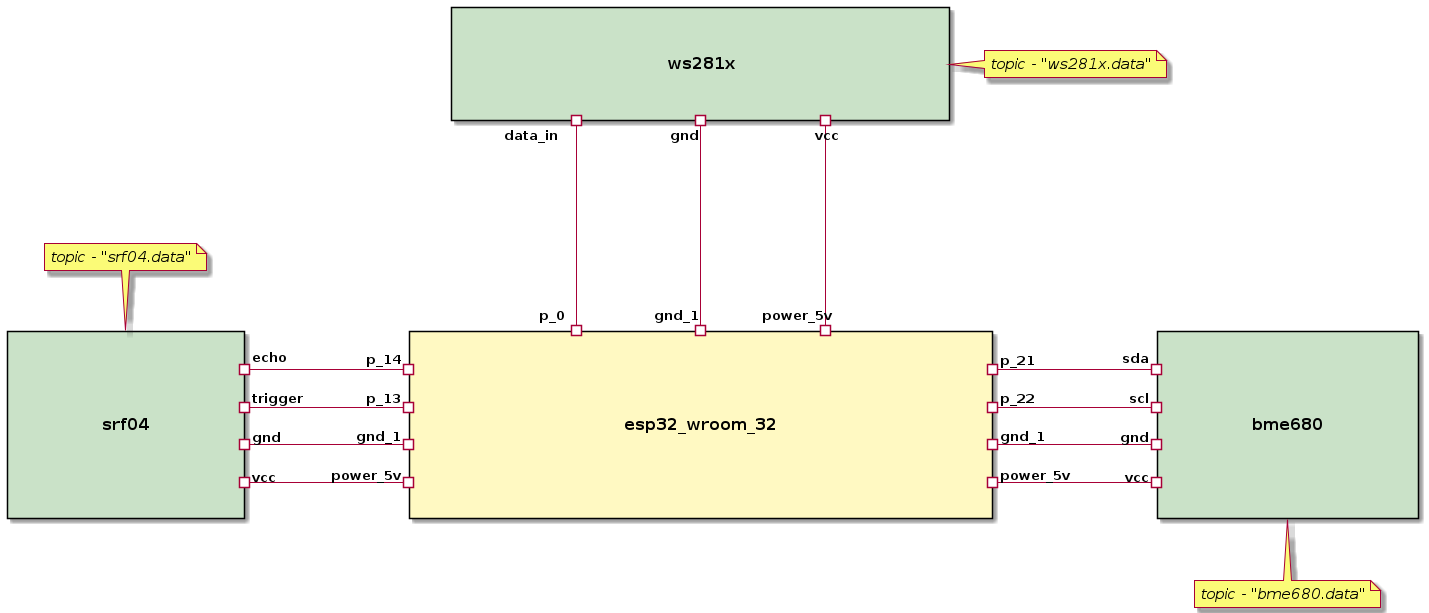
\includegraphics[width=1.0\textwidth]{./images/chapter6/example1a.png}
	\caption[\textit{Συνδεσμολογία μεταξύ των συσκευών}.]{\textit{Συνδεσμολογία μεταξύ των συσκευών}.}
	\label{fig:example_connections}
\end{figure}

Με την εκτέλεση των παραχθέντων αρχείων ξεκινάει ο έλεγχος των περιφερειακών. Υπάρχουν τα ακόλουθα τερματικά:

\begin{itemize}
	\item srf04.data: Εδώ κοινοποιούνται οι μετρήσεις από το sonar (απόσταση)
	\item bme680.data: Εδώ κοινοποιούνται οι μετρήσεις από τον αισθητήρα περιβάλλοντος (θερμοκρασία, υγρασία, πίεση)
	\item ws281x.data: Εδώ μπορούν να κοινοποιηθούν τιμές RGB, τις οποίες λαμβάνει ο ενεργοποιητής με τα LED και άρα τα ανάβει σύμφωνα με το δοσμένο χρώμα
\end{itemize}

\begin{figure}[!ht]
	\begin{subfigure}{\textwidth}
		\centering
		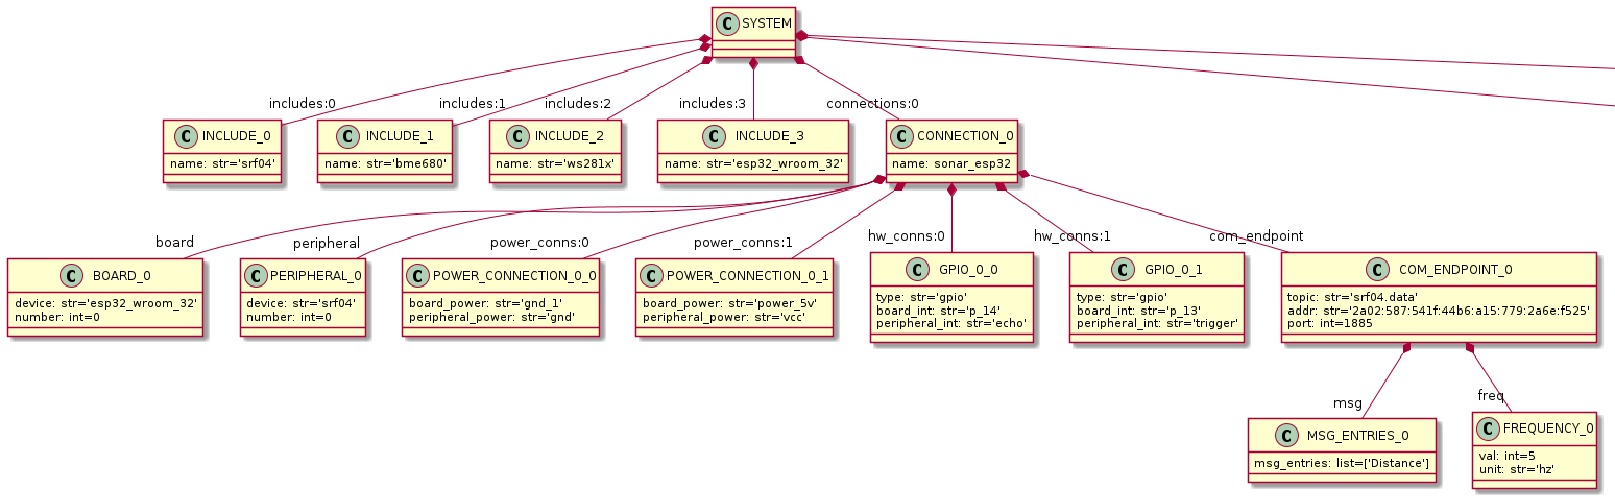
\includegraphics[width=\textwidth]{./images/chapter6/example1b1.png}
		\caption{Στοιχεία σύνδεσης με σόναρ}
		\label{fig:exmpl_1b1}
	\end{subfigure}
	
	\medskip
	
	\begin{subfigure}{\textwidth}
		\centering
		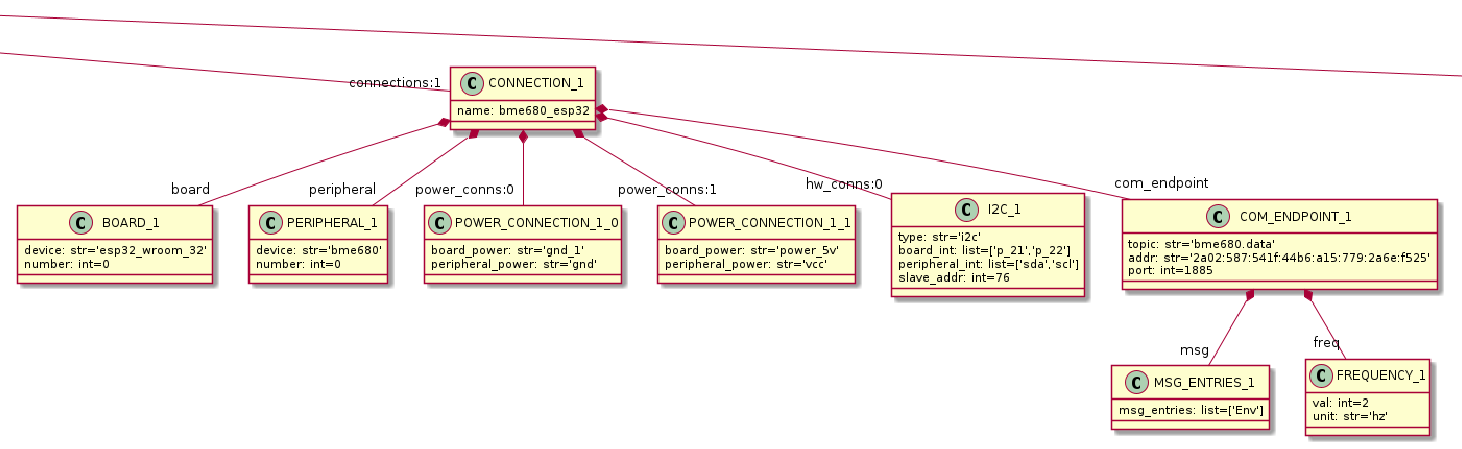
\includegraphics[width=\textwidth]{./images/chapter6/example1b2.png}
		\caption{Στοιχεία σύνδεσης με αισθητήρα περιβάλλοντος}
		\label{fig:exmpl_1b2}
	\end{subfigure}
	
	\medskip
	
	\begin{subfigure}{\textwidth}
		\centering
		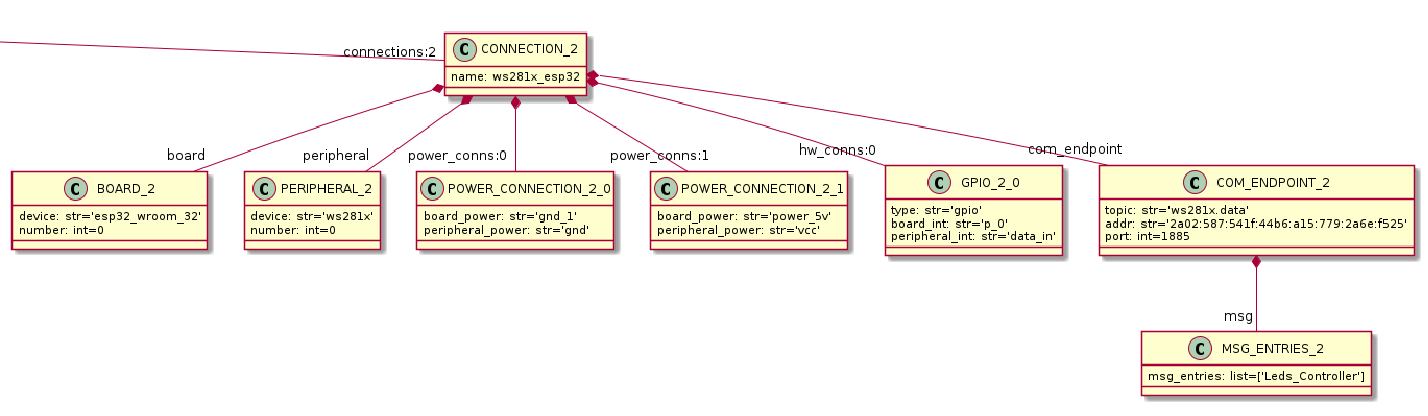
\includegraphics[width=\textwidth]{./images/chapter6/example1b3.png}
		\caption{Στοιχεία σύνδεσης με ενεργοποιητή LED}
		\label{fig:exmpl_1b3}
	\end{subfigure}
	
	\caption{Απεικόνιση μοντέλου συνδέσεων}
	\label{fig:connections_model}
\end{figure}

\newpage